\section{Auswertung}
\label{sec:Auswertung}
\subsection{Vorbereitende Versuche}
Als Vorbereitende Versuche wird die Schallgeschwindigkeit über die Resonanzfrequenzen bestimmt und es wird ein Vergleich gezogen
zwischen der Datennahme mittels Osziloskop und mittels dem Programm \texttt{SpectrumSLC}.
\subsubsection{Bestimmung der Schallgeschwindigkeit}
Aus \eqref{??}[$\lambda$ abhängig von d] kann die Schallgeschwindigkeit über die Differenz der Resonanzfrequenzen
bestimmt werden. Hierfür werden diese gegen die Länge der Röhren aufgetragen. Die Länge der Röhren ist bekannt, da immer Röhren 
der gleichen Länge hinzugefühgt werden.
\FloatBarrier
\begin{table}
    \centering
    \caption{Messwerte für die Bestimmung der Schallgeschwindigkeit}
    \label{tab:Schallgeschwindigkeit}
    \begin{tabular}{c c c c}
        \toprule
        Länge /\SI{}{\milli\meter}& erste Resonanz /\SI{}{\kilo\hertz} & zweite Resonanz /\SI{}{\kilo\hertz}& Differenz /\SI{}{\kilo\hertz}\\
        \midrule
        $\num{50}$&$\num{6.87}$&$\num{10.28}$&$\num{3.41}$\\
        $\num{100}$&$\num{6.89}$&$\num{8.6}$&$\num{1.71}$\\
        $\num{150}$&$\num{6.895}$&$\num{8.05}$&$\num{1.16}$\\
        $\num{200}$&$\num{6.897}$&$\num{7.759}$&$\num{0.86}$\\
        $\num{250}$&$\num{6.9}$&$\num{7.59}$&$\num{0.69}$\\
        $\num{300}$&$\num{6.9}$&$\num{7.477}$&$\num{0.58}$\\
        \bottomrule
    \end{tabular}
\end{table}
\FloatBarrier
Durch die Messwerte aus \ref{tab:Schallgeschwindigkeit} wird die Funktion
\begin{equation*}
    f(x) = a \frac{1}{x} + b
\end{equation*}
gefittet.\\
Mit der Gleichung 
\begin{equation*}
    nc = 2df +b =2a+b
\end{equation*}
kann die Schallgeschwindigkeit bestimmt werden.
\FloatBarrier
\begin{figure}
    \caption{Messwerte und Fitfunktion für die Bestimmung der Schallgeschwindigkeit}
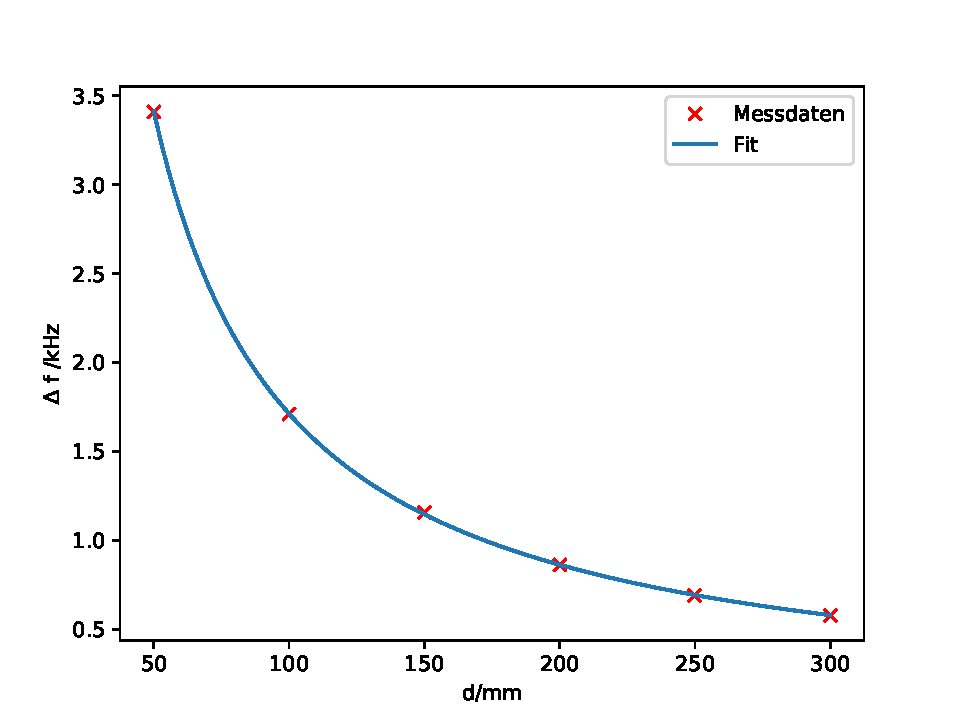
\includegraphics[width = \textwidth]{figure/Schallgeschwindigkeit.pdf}
\end{figure}
\FloatBarrier
Die Parameter der Funktion sind:
\begin{equation*}
    a= \num{169.9(3)}\\
    b= \num{0.013(3)}
\end{equation*}
Daraus kann der Wert $c=\SI{339.8(7)}{\meter\per\second}$ bestimmt werden.

\subsubsection{Vergleich der Datennahme}
Um die beiden Methoden der Datennahme zu testen wird das Spektrum des Zylinders vermessen.
Hierbei wird die Anzahl der Zylinder schrittweise von eins auf sechs erhöht.
\FloatBarrier
\begin{figure}
    \begin{minipage}[b]{.4\linewidth} % [b] => Ausrichtung an \caption
        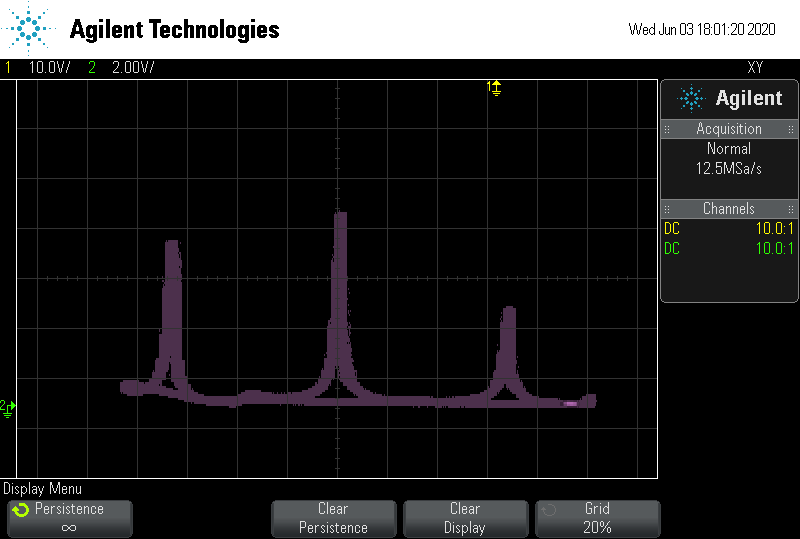
\includegraphics[width=\linewidth]{figure/1Zylinder.png}
        \vspace*{0.008cm}
        \caption{Spektrum von einem Zylinder\\ mittels Osziloskop}
     \end{minipage}
     \hspace{.1\linewidth}% Abstand zwischen Bilder
     \begin{minipage}[b]{.4\linewidth} % [b] => Ausrichtung an \caption
        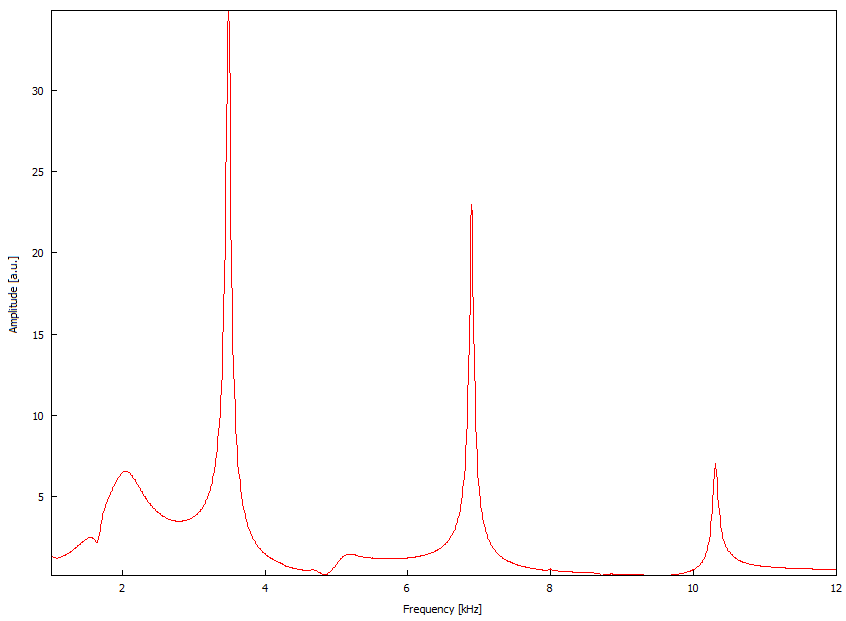
\includegraphics[width=\linewidth]{figure/1_Zylinder.png}
        \caption{Spektrum von einem Zylinder\\ mittels \texttt{SpectrumSLC}}
     \end{minipage}
\end{figure}
%\FloatBarrier
%\FloatBarrier
\begin{figure}
    \begin{minipage}[b]{.4\linewidth} % [b] => Ausrichtung an \caption
        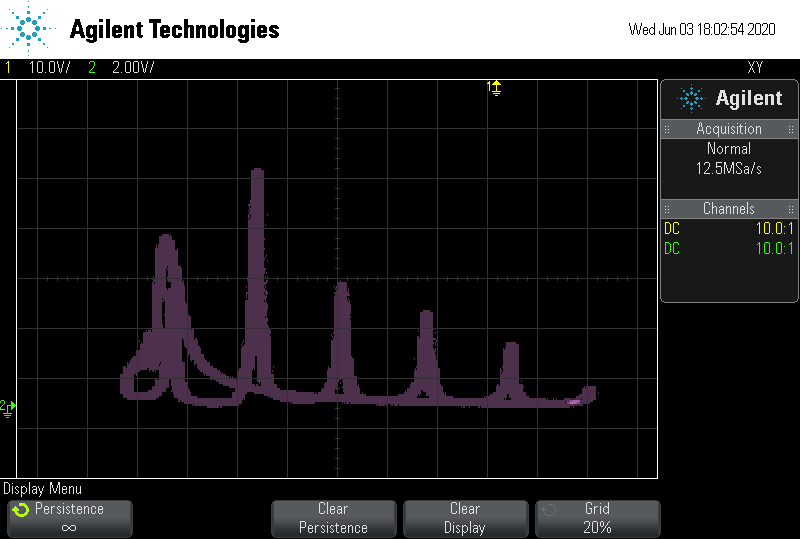
\includegraphics[width=\linewidth]{figure/2Zylinder.png}
        \vspace*{0.008cm}
        \caption{Spektrum von zwei Zylindern\\ mittels Osziloskop}
     \end{minipage}
     \hspace{.1\linewidth}% Abstand zwischen Bilder
     \begin{minipage}[b]{.4\linewidth} % [b] => Ausrichtung an \caption
        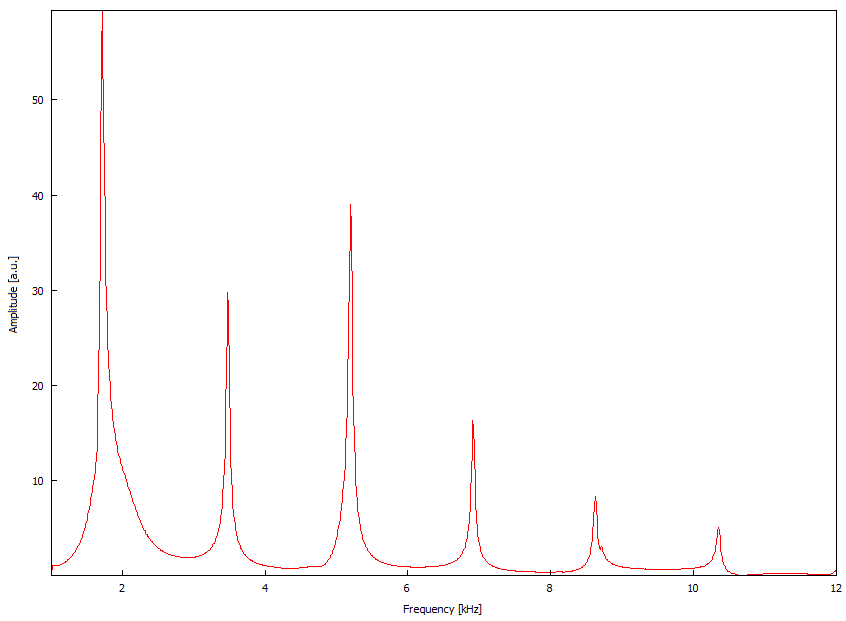
\includegraphics[width=\linewidth]{figure/2_Zylinder.png}
        \caption{Spektrum von zwei Zylindern\\ mittels \texttt{SpectrumSLC}}
     \end{minipage}
\end{figure}
%\FloatBarrier
%\FloatBarrier
\begin{figure}
    \begin{minipage}[b]{.4\linewidth} % [b] => Ausrichtung an \caption
        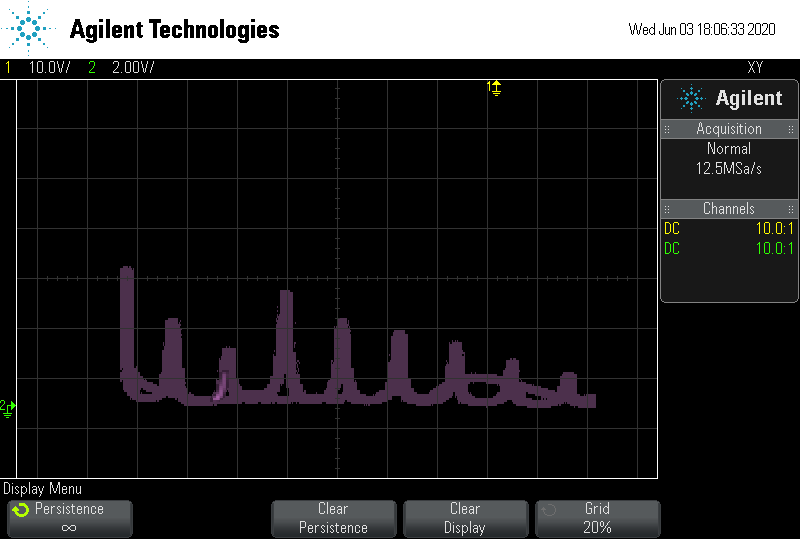
\includegraphics[width=\linewidth]{figure/3Zylinder.png}
        \vspace*{0.008cm}
        \caption{Spektrum von drei Zylindern\\ mittels Osziloskop}
     \end{minipage}
     \hspace{.1\linewidth}% Abstand zwischen Bilder
     \begin{minipage}[b]{.4\linewidth} % [b] => Ausrichtung an \caption
        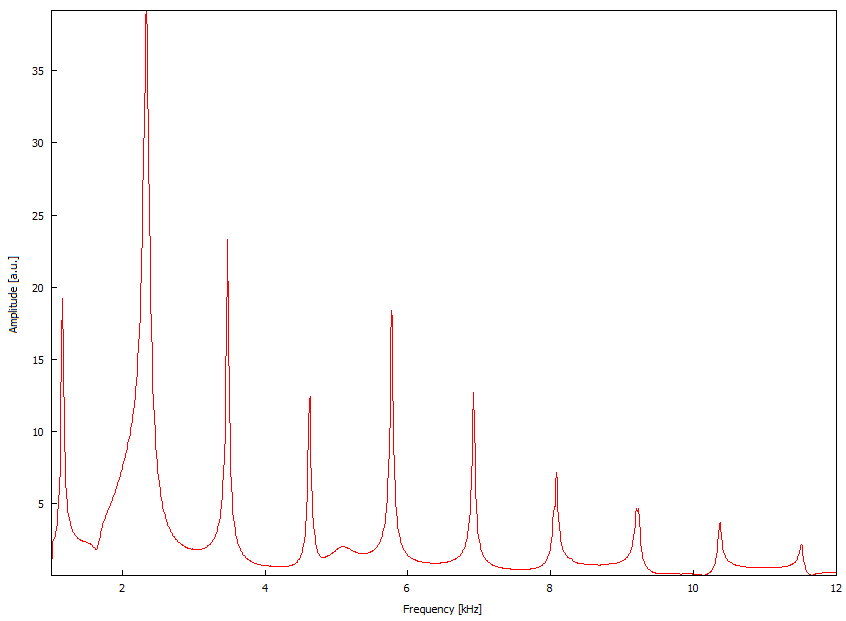
\includegraphics[width=\linewidth]{figure/3_Zylinder.png}
        \caption{Spektrum von drei Zylindern\\ mittels \texttt{SpectrumSLC}}
     \end{minipage}
\end{figure}
%\FloatBarrier
%\FloatBarrier
\begin{figure}
    \begin{minipage}[b]{.4\linewidth} % [b] => Ausrichtung an \caption
        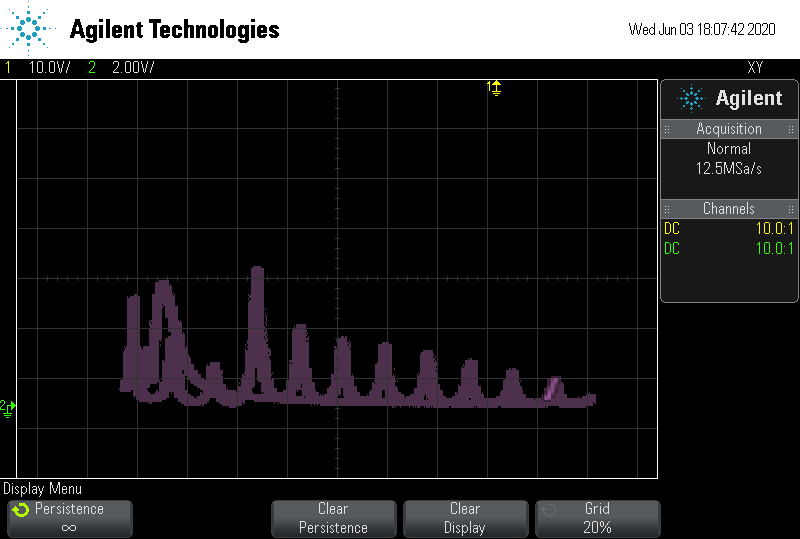
\includegraphics[width=\linewidth]{figure/4Zylinder.png}
        \vspace*{0.008cm}
        \caption{Spektrum von vier Zylindern\\ mittels Osziloskop}
     \end{minipage}
     \hspace{.1\linewidth}% Abstand zwischen Bilder
     \begin{minipage}[b]{.4\linewidth} % [b] => Ausrichtung an \caption
        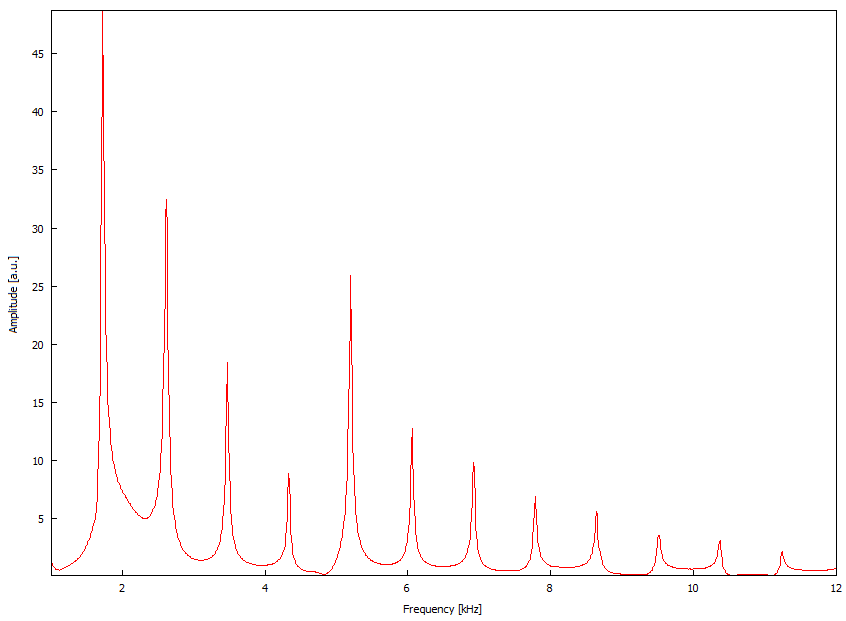
\includegraphics[width=\linewidth]{figure/4_Zylinder.png}
        \caption{Spektrum von vier Zylindern\\ mittels \texttt{SpectrumSLC}}
     \end{minipage}
\end{figure}
%\FloatBarrier
%\FloatBarrier
\begin{figure}
    \begin{minipage}[b]{.4\linewidth} % [b] => Ausrichtung an \caption
        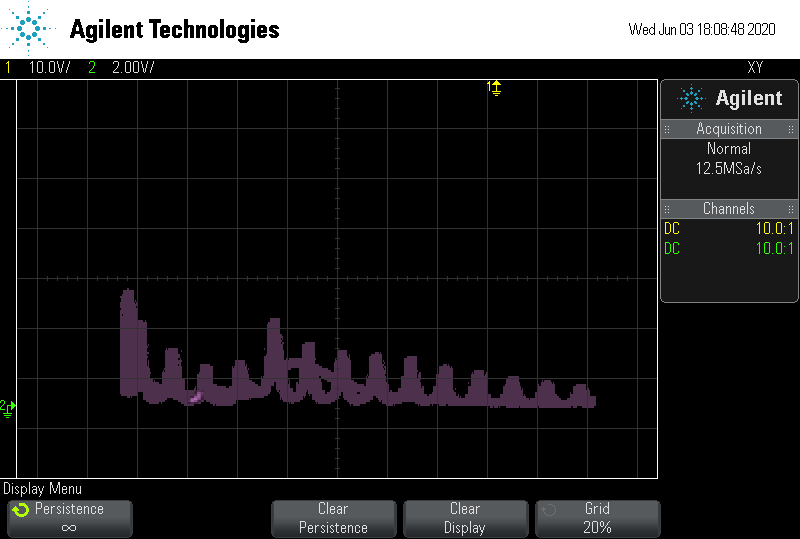
\includegraphics[width=\linewidth]{figure/5Zylinder.png}
        \vspace*{0.008cm}
        \caption{Spektrum von fünf Zylindern\\ mittels Osziloskop}
     \end{minipage}
     \hspace{.1\linewidth}% Abstand zwischen Bilder
     \begin{minipage}[b]{.4\linewidth} % [b] => Ausrichtung an \caption
        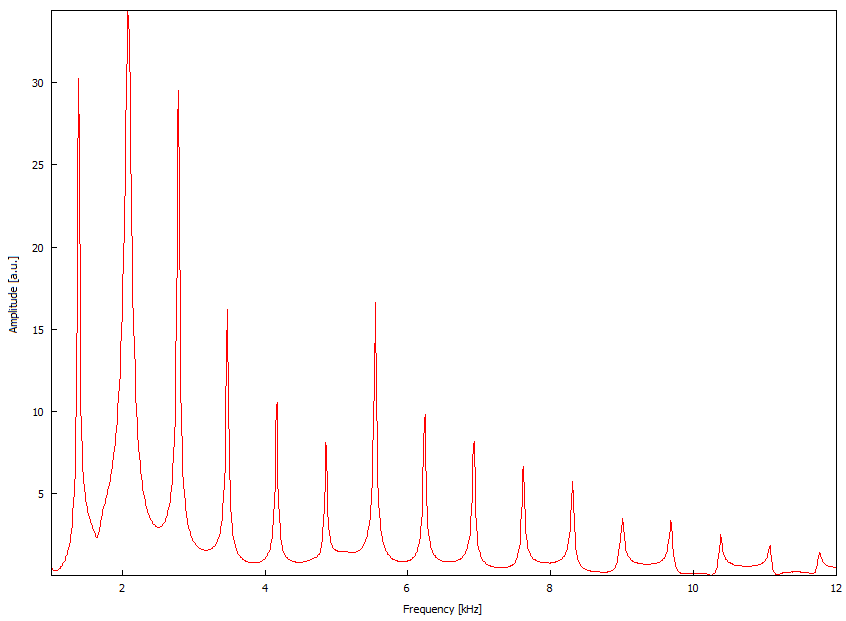
\includegraphics[width=\linewidth]{figure/5_Zylinder.png}
        \caption{Spektrum von fünf Zylindern\\ mittels \texttt{SpectrumSLC}}
     \end{minipage}
\end{figure}
%\FloatBarrier
%\FloatBarrier
\begin{figure}
    \begin{minipage}[b]{.4\linewidth} % [b] => Ausrichtung an \caption
        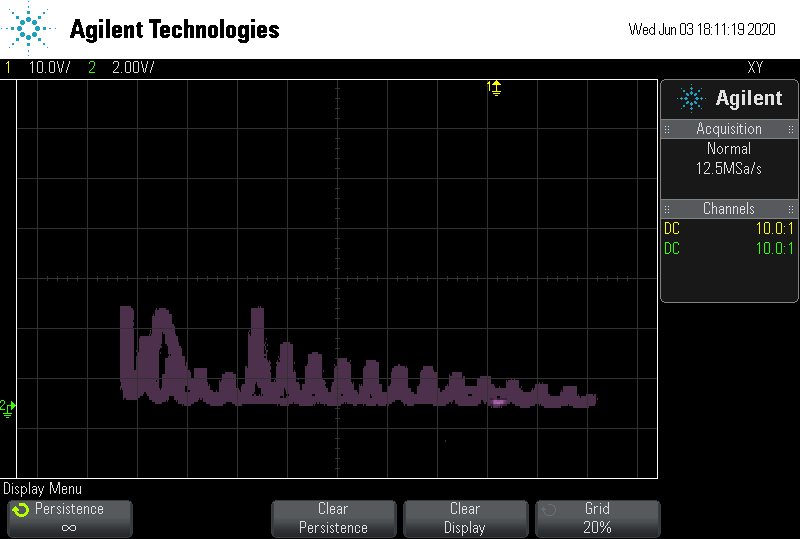
\includegraphics[width=\linewidth]{figure/6Zylinder.png}
        \vspace*{0.008cm}
        \caption{Spektrum von sechs Zylindern\\ mittels Osziloskop}
     \end{minipage}
     \hspace{.1\linewidth}% Abstand zwischen Bilder
     \begin{minipage}[b]{.4\linewidth} % [b] => Ausrichtung an \caption
        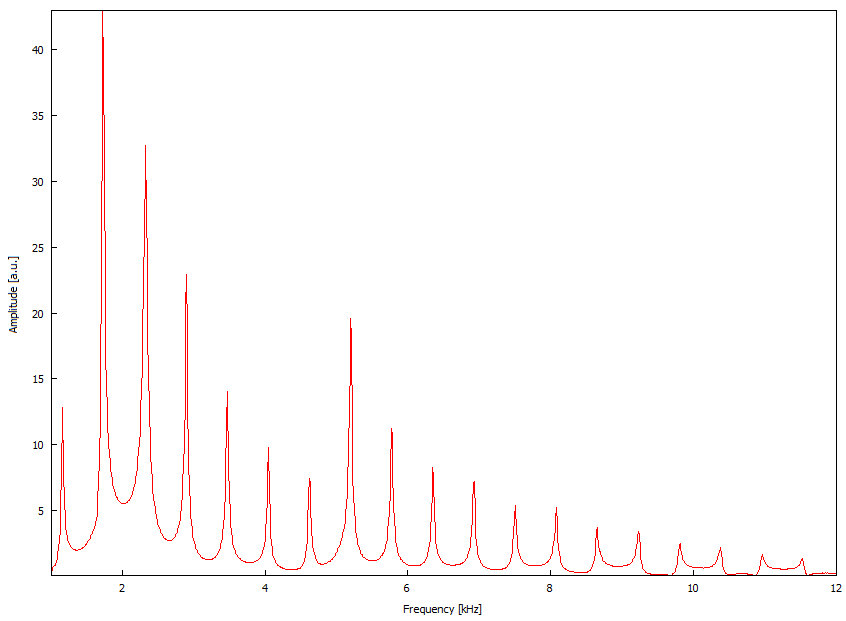
\includegraphics[width=\linewidth]{figure/6_Zylinder.png}
        \caption{Spektrum von sechs Zylindern\\ mittels \texttt{SpectrumSLC}}
     \end{minipage}
\end{figure}
\FloatBarrier

Wie an den Bildern erkannt werden kann, ist das Programm \texttt{SpectrumSLC} präzieser. Dazu kommt noch, dass das Programm die 
Daten abspeichert. Das kann die Auswertung der folgenden Messreihen vereinfachen.

\subsection{Das Wasserstoffmodel}
Für den ersten Versuch dieser Messreihe, sollen die Frequenzen von \SI{100}{\hertz} bis \SI{10}{\kilo\hertz} vermessen werden.
Die Resonanzfrequenzen sind in Tabelle \ref{tab:Resonanzfrequenzen} aufgelistet.
\FloatBarrier
\begin{table}
    \centering
    \caption{Messwertte für die Bestimmung der Ordnung der Resonanzfrequenz}
    \label{tab:Resonanzfrequenzen}
    \begin{tabular}{c c c c}
        \toprule
        Ordnung&Resonanzfrequenz /\SI{}{\kilo\hertz} &Amplitude /\SI{}{\milli\volt}& Phasenverschiebung /\SI{}{\degree}\\
        \midrule
        $\num{1}$&$\num{0.4376}$&$\num{160}$&$\num{0}-  \num{30}$\\
        $\num{2}$&$\num{2.3164}$&$\num{150}$&$\num{-20}-\num{4}$\\
        $\num{3}$&$\num{3.7095}$&$\num{150}$&$\num{-20}-\num{0}$\\
        $\num{4}$&$\num{5.0074}$&$\num{160}$&$\num{-20}-\num{0}$\\
        $\num{5}$&$\num{6.2361}$&$\num{160}$&$\num{-20}-\num{0}$\\
        $\num{6}$&$\num{6.5908}$&$\num{160}$&$\num{-20}-\num{4}$\\
        $\num{7}$&$\num{7.4648}$&$\num{160}$&$\num{-15}-\num{7}$\\
        $\num{8}$&$\num{8.0705}$&$\num{165}$&$\num{-20}-\num{0}$\\
        $\num{9}$&$\num{8.6602}$&$\num{170}$&$\num{-30}-(\num{-5})$\\
        $\num{10}$&$\num{9.5068}$&$\num{170}$&$\num{-30}-(\num{-5})$\\
        $\num{11}$&$\num{9.8462}$&$\num{175}$&$\num{-15}-\num{3}$\\
        \bottomrule
    \end{tabular}
\end{table}
\FloatBarrier
Die Resonanzen können auch mittels des Frequnezspektrometers dargestellt werden.
\FloatBarrier
\begin{figure}
    \caption{Frequnezspektrum des Kugelresonators}
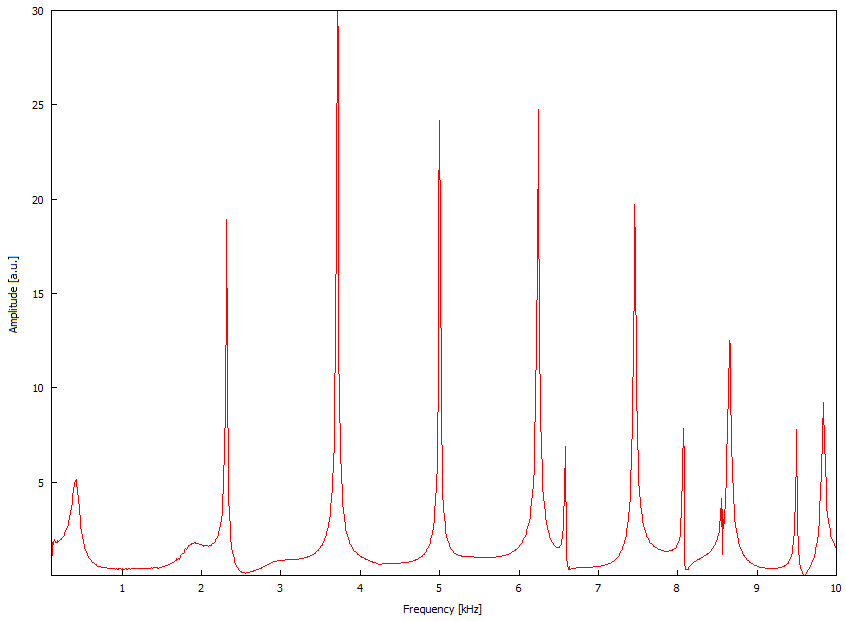
\includegraphics[width = \textwidth]{figure/Kugelresonanzspektrum.png}
\end{figure}

